\chapter{General-purpose programming of GPUs}
\label{chap:gpgpu}

The contents in this section is based on a text previously written by
Martin Dybdal, one of the authors (see \cite{dybdal2011opencl}).

GPUs show a high degree of data parallelism, which makes them
economical worthwhile for many domains in both the sciences and the
industry, as this is a characteristic of problems in these
domains. GPUs efficiency originate from their \textit{single
  instruction, multiple data}-architecture (SIMD), where a set of
computation units executes the same program on each their own data
item. In this chapter we will look at the architecture of a modern
NVIDIA GPU and introduce the necessary concepts.

% \section{Programming interfaces}
% Originally, the only programming interfaces for GPUs were based on
% concepts such as textures and shader programs. Applications outside
% the graphics domain had to be encoded to fit the models of graphics
% programming interfaces such as OpenGL or DirectX and developers needed
% deep knowledge about the GPU-architecture \cite{nvidia2009fermi}.

% Several frameworks has since been developed for GPGPU
% programming. NVIDIA developed CUDA for its line of graphics cards and
% AMD/ATI developed the Stream SDK (initially called ``Close to metal'')
% for their cards. To break with the situation where there was no
% portable interface for GPU-programming, Apple took initiative to the
% creation of OpenCL. OpenCL is an open standard for programming
% heterogeneous systems with several kinds of processors, both CPUs and
% GPUs. There are OpenCL implementations available for, newer NVIDIA and
% ATI GPUs, the x86 and x86\_64 CPU-architectures and the Cell
% processor.

% Although CUDA and OpenCL are more general than the graphics frameworks
% used previously, they are still low-level interfaces in today's
% terms. The programmer himself is responsible for administering memory
% usage himself and manually moving data between main memory and GPU
% memory. To write even simple programs it is large amounts of
% surrounding code are necessary. This includes: initialization of
% OpenCL and connected devices, compilation of GPU specific code,
% invocation of GPU-functions (kernels) and data-transfers to and from
% the GPU. To use the GPU effectively, a certain level of knowledge
% about the architecture of graphics processing units is also
% necessary. For instance, using the local caches incorrectly or
% misaligning memory accesses between work items can cause huge
% performance penalties.

\begin{figure*}
  \centering
  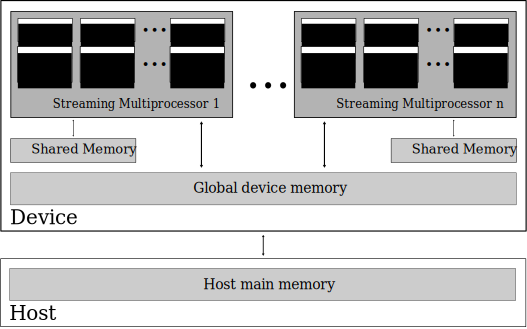
\includegraphics[width=\textwidth]{graphics/cuda-structure}
  \vspace{2mm}
  \caption{CUDA GPU terminology: Host, devices, streaming
    multiprocessors and CUDA cores. The arrows show the possible path
    of data movement. The host can command movement of data to and
    from host memory and device memory. Kernel code is responsible for
    moving data between global memory, shared memory and registers.}
  \label{fig:gpu_terminology}
\end{figure*}

\section{CUDA}
The execution of a GPU program has to be conducted by an accompanied
program executing on the CPU. The traditional CPU is referred to as
the \textit{host} and the GPU is called the \textit{device}. Other
concepts such as pointers or arrays are often prefixed with either of
these to specify where they reside.

An CUDA device is divided into streaming multiprocessors (SM, or just
``multiprocessor''), which are in turn divided into individual CUDA
cores. CUDA cores performs the actual computation on a GPU. How these
concepts are related is shown in Figure \ref{fig:gpu_terminology}.
Since modern GPUs contains hundreds or thousands of cores, GPU
programs must be written such that their work can be executed
independently and in parallel on as many of these cores as possible. A
single thread of execution on a CUDA core is the smallest unit of work
on a GPU. These threads are arranged into equal sized groups called
\textit{blocks} and blocks are arranged into an $3$-dimensional
grid. A \textit{block} is executed on a single multiprocessor, which
provides shared memory accessible from all its cores.

Programming a GPU is done by writing \textit{kernel programs} or
simply \textit{kernels}. A kernel specifies the work done by a single
thread of the complete problem. It is the task of kernel program
itself, to find the subset of the data that it has to work on. That
is, all executions of the kernel receives exactly the same arguments,
but the kernel can query where it is located in its block and grid of
blocks and use this information to select the appropriate part of the
input. When executing tasks on CUDA devices, it is common to divide
the problem into logically separate kernels scheduling them as their
dependencies are met.

\todo{synchronization in CUDA}

\todo{describe memory allocation in CUDA: specific versions of malloc
  and free for GPU memory and cudaMemcpy to transfer data to and from the host}

\section{Hardware}
\label{sec:gpu_hardware}
In this section we will introduce the GPU devices produced by NVIDIA,
as it is GPUs from this vendor we have available at the department.

The architecture of NVIDIAs latest line of GPGPU devices is named
Kepler. The current Kepler based GPUs consists of up to 1536 CUDA
cores grouped into \textit{streaming multiprocessors} (SM) of 192
cores each. Shared between all SMs is an L2 Cache (512 KB) of global
memory \cite{nvidia2012gtx680}. Figure \ref{fig:kepler_sm} shows the
structure of a streaming multiprocessor in the Kepler
architecture. All 192 cores share the same register file (in the top)
and 64 KB of local memory (at the bottom) is used both as L1 cache and
shared memory between cores of the SM. The amount of memory used as
cache and as shared memory is configurable.

\begin{figure}
  % floatflt package?
  \centering
  \vspace{5mm}
  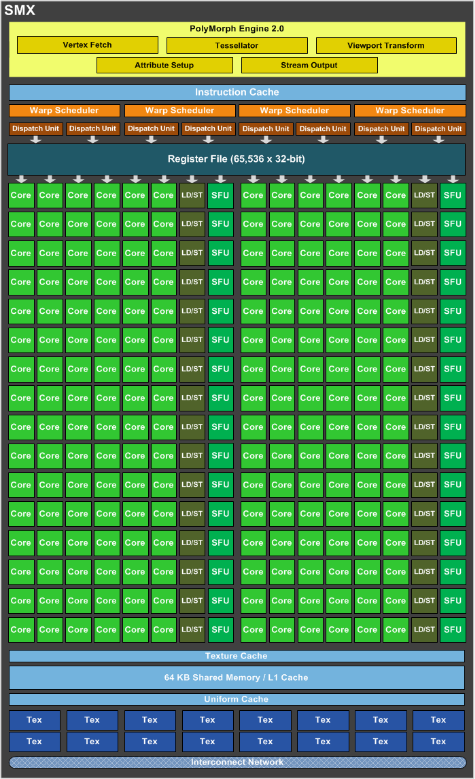
\includegraphics[width=\textwidth]{graphics/nvidia_kepler_k104_sm}
  \vspace{4mm}
  \caption{A single streaming multiprocessor of a Kepler K104 GPU. The
    illustration is borrowed from NVIDIAs K104 whitepaper
    \cite{nvidia2012keplerk104}.}
  \label{fig:kepler_sm}
\end{figure}

When executing a grid of CUDA blocks on a Kepler architecture GPU,
each block is assigned to a single SM (each SM can process several
blocks). Each block is partitioned into \textit{warps} which are
groups of 32 threads, which are scheduled on the 192 CUDA cores of the
streaming multiprocessor. Notice that the 192 CUDA cores does not
divide evenly into groups of 32 threads (which was common on previous
architectures, such as NVIDIA Fermi).
\todo{explain why this is the case}

All threads in a \textit{warp} always executes exactly the same
instruction, this is called \textit{SIMD}, single instruction,
multiple data. Moreover, when warps are executed by a SM it can
execute two warps from the same block simultaneously, as each SM have
access to two schedulers and the register file can be used for both of
the two warps independently. This is called \textit{SIMT} (single
instruction, multiple thread) as two threads are executed on the same
processor simultaneously. Each streaming multiprocessor can be
assigned a certain number of warps, which it switches between
executing. This is useful for hiding latency endured by memory access
or data dependencies between instructions.

\subsection{Optimization considerations}
Determining how the grid of threads are partitioned into blocks are of
importance when optimizing for fast execution. There should at least
be as many blocks as there are streaming multiprocessor, to avoid
having a stalled processor. If blocks have to wait for synchronization
with other blocks it might also be beneficial to have more than one
block per SM. In a NVIDIA presentation on \textit{OpenCL Optimization}
\cite{nvidia2009opencloptimization}, it is recommended to spawn at
least 100 blocks per streaming multiprocessor (for large problems), if
the program should scale well on future devices.

The number of warps should also be considered, as having enough
available warps can hide latency from memory transactions. Accessing
global memory can stall a streaming multiprocessor for 400-600 cycles,
where as local memory access only partakes a couple of cycles
\cite{nvidia2009opencloptimization}. This is not the largest
bottleneck though, as GPUs are presently connected to the host through
PCI Express ports which have a throughput limit of 8-16 GB/s
(depending on the generation of the device). Accessing global memory
on the device can be done at 150 GB/s. The bottleneck of this has been
observed by the hardware vendors and AMD has developed a line of
products called \textit{AMD
  Fusion}\footnote{\url{http://fusion.amd.com/}} which combines the
CPU and the GPU into the same chip. NVIDIA has also announced plans to
develop such \textit{Accelerated Processing Units}, which is the
general term for this fusion of processor technologies.

It is not always good for efficiency to have large blocks with many
warps, as each streaming multiprocessor has a limited amount of
registers and local memory. All threads currently executed on a SM
shares the same register-file, and blocks are only assigned to a SM if
there are enough available registers for all of its threads. Thus, to
get optimal occupancy, blocks must be sized such that the size of the
register-file is divisible by the total amount of needed registers. An
occupancy calculator created by NVIDIA is available as a spreadsheet
on the NVIDIA
website\footnote{\url{http://developer.download.nvidia.com/compute/cuda/CUDA_Occupancy_calculator.xls}}.

\subsection{Memory access patterns}
Accessing global device memory are always done in segments of 32, 64
or 128 bytes, and these accesses must be aligned such that segments
are placed in physical device memory with a segment, starting on
addresses that are a multiple of the segment size
\cite{nvidia2010cudaguide}. When a warp gets executed, the memory
transaction of individual threads are coalesced such that the
needed memory can be fetched by a single memory transaction. To
minimize the number of memory transactions, it is thus important to
write kernels, such that nearby threads which are scheduled in the
same warp, will access memory in the same memory region. Previous
architectures had strict rules for how data accesses should be
distributed. If simultaneous operations on memory from a warp was out
of sequence on such a device, all the operations was performed as
separate memory transactions. The same would happen if accesses were
not aligned correctly. With the Fermi architecture, accesses are
cached such that out of order accesses can be coalesced into single
transactions and misalignments can be handled as long as they do not
cross 128 byte boundaries. If a segment of 32 bytes are accessed such
that this access overlap two physical 32-byte segments, the 64-byte
segment containing both of them are loaded from global memory instead.

These considerations are explained in detail in ``The CUDA C
Programming Guide'' by NVIDIA \cite{nvidia2010cudaguide} and the guide
``AMD Accelerated Parallel Processing OpenCL\texttrademark''
\cite{amd2011opencl} covers the same concepts for GPU devices by AMD.


%%% Local Variables:
%%% mode: latex
%%% TeX-master: "master"
%%% End:
